%! TEX root = ../thesis.tex
\section{Probabilistic Choice Models}
\label{in:sec:models}

\subsection{A Brief History}
% Why studying choices to study human behaviour is important and useful
% - Long literature from psychometrics and econometrics
% - New methods enabled by computer science to process large-scale datasets
% - Example: The use of preference learning for virtual democracy
% - Example: Ranking from discrete comparisons
% - Example: Search

% Describe work of Thurstone and Zermelo.
% In the psychometrics community.
The history of studying choices to understand human behaviour has its roots in the 1920s in the psychometrics community.
\citet{thurstone1927law} pioneered the ``law of comparative judgment'' that established the methodology of measuring the perception of physical \emph{stimuli} (\textit{e.g.}, the weight of different objects) from pairwise comparisons.
That same year, he used his new approach~\citep{thurstone1927method}, today known as the \emph{probit model}, to study people's perception of the seriousness of crimes, a notion for which no physical scale exists.
Almost concurrently, \citet{zermelo1928berechnung} proposed a similar model, known as the \emph{logit model}, to rank chess players from outcomes of matches\footnote{This approach is still used today by the World Chess Federation~\citep{elo1978rating}.}.
Zermelo's model was then independently rediscovered in the early 1950s in the statistics community by~\citet{bradley1952rank}.

% Describe work of Marschak, Luce (IIA), and McFadden (conditional logit)
In the late 1950s, \citet{marschak1959binary} introduced Thurstone's work to the econometrics community by interpreting the psychological stimuli of Thurstone's model as economic \emph{random utility}.
In parallel, \citet{luce1959individual} proposed his \emph{choice axiom} and the hypothesis of \emph{independence of irrelevant alternatives} (IIA) that states that the relative comparison of two alternatives is unaffected by additions and subtractions of other alternatives.
In other words, it assumes that the alternatives are uncorrelated.
This property enabled Luce to extend the logit model to multi-way comparisons.
This extension was also proposed by~\citet{mcfadden1973conditional} to introduce the \emph{multinomial logit model}\footnote{This model was first introduced as the \emph{conditional logit model}.} from a random utility viewpoint.

% Research between 1970 until today
% Unification and new models to relax the IIA hypothesis and account for correlation between alternatives
The subsequent decades were dedicated to extending discrete-choice models.
In particular, to relax the (rather restrictive) IIA hypothesis, \citet{ben1973structure} and \citet{williams1977formation} developed the \emph{nested logit model} that encodes correlation between alternatives through their joint distribution.
Similarly, \citet{boyd1980effect} and \citet{cardell1980measuring} developed the \emph{mixed logit model}, which encodes correlation by assigning a probability distribution to the parameters of the (multinomial) logit model~\citep{hensher2003mixed}.
Some efforts were also deployed by~\citet{yellot1977relationship} to unify the different formulations of the logit model.
% Ranking
In parallel, pairwise-comparison data started to be exploited for \emph{ranking}~\citep{ford1957solution,buehlmann1963pairwise,plackett1975analysis,wauthier2013efficient,negahban2017rank}, a model often referred to as the \emph{Plackett-Luce model}~\citep{hensher2003mixed}.
% Inference
Research addressing the inference of discrete-choice models was also conducted for \emph{sampling and simulations}~\citep{manski1981alternative,cosslett1981efficient}, \emph{maximum likelihood estimation}~\citep{hastie1998classification,hunter2004mm,maystre2015fast,vojnovic2016parameter}, and \emph{Bayesian inference}~\citep{guiver2009bayesian,caron2012efficient,houlsby2012collaborative}.

Today, the availability of unprecedented computational power and of large-scale datasets has enabled new applications of discrete-choice models.
% Describe its use in reinforcement learning.
In reinforcement learning, \citet{sadigh2017active} and~\citet{christiano2017deep} propose to use pairwise-comparison models to incorporate feedback from human supervisors into the reward function.
% Describe the work of Lucas for ranking and recommendation \citet{ammar2015ranked}
\citet{ammar2015ranked} suggests using these models to make personalized recommendations.
% Describe the work of Daniyar for search.
\citet{chumbalov2020scalable} propose a search algorithm for navigating large-scale databases of complex items (\textit{e.g.}, images) from pairwise comparisons.
% Describe the work of Anson for preference learning in virtual democracy and AllOurIdeas.
To make algorithmic policies, \citet{lee2019webuildai} apply the Plackett-Luce model in a \emph{virtual democracy} setting to learn people's preferences.
\citet{noothigattu2018voting} also use this model to train autonomous vehicles to make ethical decisions.
Finally, \citet{salganik2015wiki} implemented the probit model into the online platform \emph{All Our Ideas}\footnote{\href{http://www.allourideas.org/planyc_example?guides=true}{http://www.allourideas.org}} to help the New York City Mayor’s Office of Long-Term Planning and Sustainability understand New Yorkers' preferences for developing the city sustainably.

A history of the development of discrete-choice models in econometrics is given by~\citet{mcfadden2001economic} in his Nobel-Prize lecture.
The curious reader will find more details about random utility models in the books of~\citet[Chapter~1]{train2009discrete} and~\citet[Chapter~3]{hensher2005applied}.
An introduction to probabilistic models of choice from a statistical perspective is given by~\citet[Chapter~1]{maystre2018efficient}.
In the next section, we introduce discrete-choice models from a \emph{random utility} perspective.

\subsection{Random Utility Models}

\subsubsection{Choice Set}
% - Definition and notation of a choice set.
% - Three characteristics: mutually exclusive, exhaustive, finite
Discrete-choice models capture people's preferences that drive their choices.
When facing a set of (at least two) alternatives, a decision-maker chooses one of the alternatives over the other(s).
This set of alternatives is defined as the \emph{choice set}.

\begin{definition}[Choice Set]
	Given the set of all possible alternatives~$\mathcal{A}$, the \emph{choice set}~$\mathcal{C} \subseteq \mathcal{A}$ is the set of alternatives faced by a decision-maker.
	It has the following three characteristics:
	\begin{enumerate}
		\item The alternatives are \emph{mutually exclusive}.
		\item The choice set $\mathcal{C}$ is \emph{exhaustive}.
		\item The number of alternatives is \emph{finite}.
	\end{enumerate}
\end{definition}

The exclusiveness of alternatives means that, when choosing alternative $i \in \mathcal{C}$, the other alternatives of $\mathcal{C}$ are left aside.
The exhaustiveness of the choice set means that the decision-maker faces all possible alternatives at decision time.
Finally, the number of alternatives must be finite:
The decision-maker can count the alternatives.

The first two characteristics are not restrictive, because it is always possible to add artificial alternatives.
For example, if $\mathcal{C} = \{i, j\}$, exclusiveness can be ensured by adding a third alternative $k = \text{"choose $i$ and $j$"}$.
This enables the decision-maker to choose both alternatives at the same time.
Similarly, exhaustiveness can be ensured by adding another alternative $l = \text{"none of the alternatives"}$.
This enables the decision-maker to choose none of the alternatives, hence making the choice set exhaustive.

The third characteristic is, however, restrictive.
A finite number of alternatives is actually the defining characteristic of discrete-choice models.
This contrasts with regression models, in which the target variable is continuous, hence the number of alternatives is infinite.
The choice set can also vary for each choice faced by a decision-maker.
For example, $\mathcal{C}_1 = \{ i, j \}$ and $\mathcal{C}_2 = \{ i, j, k \}$.
This contrasts with classification models, in which the choice set, \textit{i.e.}, the domain of the target variable, is identical for every observation.
For example, in the context of email classification, $\mathcal{C}_1 = \mathcal{C}_2 = \{ \text{``spam''}, \text{``ham''} \}$.

\subsubsection{Random Utility}
% Define a random utility and the error term.
% Explain that the main assumption to be made is on the error term.

Without loss of generality, we introduce the random utility models from an econometrics viewpoint, \textit{i.e.}, by analyzing the behavior of decision-makers facing choices.
These methods can obviously be used to model other processes.
In particular, and as we will see in this thesis, they can model \emph{implicit} choices.
For example, in the context of collective-sport matches, if Team~$A$ wins against Team~$B$, then Team~$A$ is implicitly chosen over Team~$B$ (\textit{e.g.}, because it played better or had good lucky).

In econometrics, we posit that a decision-maker is rational and chooses the alternative that maximizes its personal gain.
For example, let us consider a sleepy Ph.D.\ student who needs a hot beverage in the morning in order to start working on their research.
Let~$\bm{x}_i \in \mathbf{R}^M$ be a vector of $M$ observable features that might influence a person's decision to choose alternative~$i \in \mathcal{C}$, and let $\bm{w}\in \mathbf{R}^M$ be the associated $M$-dimensional parameter vector.
In our example, the choice set is $\mathcal{C} = \{ \text{``espresso''}, \text{``cappuccino''}, \text{``Earl Grey tea''}  \}$ and the features could include the type of beverage (coffee or tea), the level of caffeine, and the preparation time.
The feature vector could also include features of the student, such as their age, their gender, and their baseline level of glucose.

It is impossible to characterize \emph{all} features that influence a decision-maker's choice. %, because this would require feature vectors of infinite size.
Therefore, we capture the effect of the unobserved features in a random noise variable~$\epsilon_i$, whose probability distribution is to be defined.
In our example, the noise could capture the effect of the atmospheric pressure on the quality of the brew and the influence of the student's personal history on their choice\footnote{The student could have a preference for Earl Grey tea because this reminds them of their grandfather.}.

To analyze the decision-maker's behaviour, economists posit that an alternative~$i$ has a \emph{random utility}~$U_i$ given by
\begin{equation*}
	U_i = \bm{x}_i\Tr \bm{w} + \epsilon_i,
\end{equation*}
and the decision-maker chooses alternative~$i$ if $U_i > U_j$, for all $j \neq i$, $i,j \in \mathcal{C}$.
Hence, the probability that a decision-maker chooses~$i$ over~$j$ is
\begin{align}
	\label{in:eq:choiceprob}
	\Prob{i \succ j} & \coloneqq \Prob{U_i > U_j}                                                  \nonumber \\
	                 & = \Prob{\bm{x}_i\Tr \bm{w} + \epsilon_i > \bm{x}_j\Tr \bm{w} + \epsilon_j} \nonumber  \\
	                 & = \Prob{\epsilon_i - \epsilon_j > \bm{x}_j\Tr \bm{w} - \bm{x}_i\Tr \bm{w}}.
\end{align}
The probability $\Prob{i \succ j}$ is called the \emph{choice probability}.
The notation ``$i \succ j$'' reads as ``alternative~$i$ is chosen over alternative~$j$'' or, equivalently, as ``$i$ wins over $j$''.
In our example, we are interested in the probability $\Prob{\text{``capuccino''} \succ \text{``espresso''}}$ that the student will choose to drink a cappuccino instead of an espresso.

From~\eqref{in:eq:choiceprob}, the characterization of a discrete-choice model depends on the researcher's hypotheses on the noise model, \textit{i.e.}, on the probability distribution that captures the unobserved features best.
Two popular choices of distribution, which we describe below, are (i) the Gaussian distribution $\DNorm{\mu, \sigma^2}$ with mean~$\mu$ and variance~$\sigma^2$, and (ii) the Gumbel distribution $\DGumbel{\mu, \beta}$ with location $\mu$ and scale $\beta$.
The probability density function of these two distributions are
\begin{align*}
	f_{\text{Gaussian}}(x) & = \frac{1}{\sigma \sqrt{2 \pi}} \exp \left[ -\frac{(x - \mu)^2}{2 \sigma^2} \right], \\
	f_{\text{Gumbel}}(x)   & = \frac{1}{\beta} \exp \{ - [z + \exp(-z)]\},
\end{align*}
where  $z = \frac{x - \mu}{\beta}$.
We show in Figure~\ref{in:fig:pdf} an example of these two distributions with $\mu = 0$ and $\sigma^2 = \beta = 1$.

\begin{figure}
	\centering
	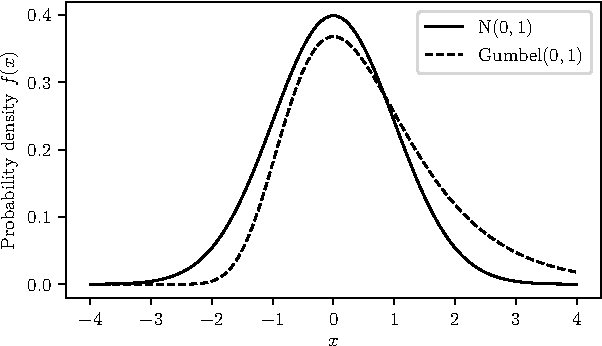
\includegraphics{in-pdf}
	\caption{Probability density functions of Gaussian and Gumbel distributions.}
	\label{in:fig:pdf}
\end{figure}

\paragraph{Probit Model}

The probit model was first introduced by~\citet{thurstone1927law} in the context of psychometrics.
In this model, the random noise is independently and identically distributed (i.i.d.) with a Gaussian distribution $\epsilon_i, \epsilon_j \sim \DNorm{0, 0.5}$.
As the difference of two Gaussian random variables is also Gaussian, \textit{i.e.}, $\epsilon_i - \epsilon_j \sim \DNorm{0, 1}$ in this special case, the choice probability for the probit model is
\begin{equation}
	\label{in:eq:probit}
	\Prob{i \succ j} = \Prob{\epsilon_i - \epsilon_j > \bm{x}_j\Tr \bm{w} - \bm{x}_i\Tr \bm{w}} = \Phi \left( \bm{x}_i\Tr \bm{w} - \bm{x}_j\Tr \bm{w} \right),
\end{equation}
where $\Phi( \cdot )$ is the cumulative distribution function of the standard normal distribution, as shown in Figure~\ref{in:fig:cdf}.
When the random utility is parameterized by only one parameter, each alternative~$i$ is represented by a one-dimensional parameter~$w_i \in \mathbf{R}$.
The feature vector $\bm{x}_i$ becomes a one-hot vector that is 0 everywhere except in~$i$, where it is 1, \textit{i.e.}, it ``selects'' the parameter associated with alternative~$i$.
Then, $U_i = \bm{x}_i\Tr \bm{w} + \epsilon_i = w_i + \epsilon_i$, and the model
\begin{equation*}
	\Prob{i \succ j} = \Phi \left( w_i - w_j \right)
\end{equation*}
is called the \emph{Thurstone model}.
The $M$ parameters~$\bm{w} = [w_1 \cdots w_M]\Tr$ represent a \emph{score} for each of the $M$~alternative.
They can be interpreted as the \emph{perceived psychological stimuli} of the alternatives and induce a natural ranking.

\begin{figure}
	\centering
	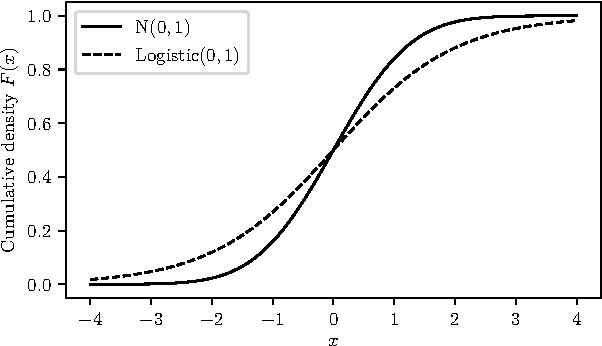
\includegraphics{in-cdf}
	\caption{Cumulative density functions of Gaussian and logistic distributions.}
	\label{in:fig:cdf}
\end{figure}

\paragraph{Logit Model}
% Define the logit model, \textit{i.e.}, the Bradley-Terry model

The logit model was introduced by~\citet{zermelo1928berechnung} and rediscovered two decades later by~\citet{bradley1952rank}.
In this model, the random noise is assumed to follow a Gumbel distribution\footnote{This distribution is also called the (Type I) extreme value distribution.} $\epsilon_i \sim \DGumbel{\mu_i, \beta_i}$ (see Figure~\ref{in:fig:pdf}).
The Gumbel distribution has the property that the difference of two Gumbel random variables $G_1$ and $G_2$ with locations $\mu_1$ and $\mu_2$, and scales $\beta_1 = \beta_2 = \beta$, follows a logistic distribution $G_1 - G_2 \sim \DLogistic{\mu', \beta'}$, whose cumulative density function is
\begin{equation*}
	F_{\text{Logistic}}(x)
	= \sigma\left(\frac{x - \mu'}{\beta'}\right)
	= \frac{1}{1 + \exp \left[ - \frac{x  - \mu'}{\beta'} \right]},
\end{equation*}
where $\mu' = \mu_1 - \mu_2$ and $\beta' = \beta$, and where $\sigma(\cdot)$ is the logistic function.
We show, in Figure~\ref{in:fig:cdf}, an example of the logistic cumulative distribution function with $\mu' = 0$ and $\beta' = 1$, which we compare with that of the standard normal distribution.

In the logit model, the random noise is assumed to be i.i.d.\ with a Gumbel distribution $\epsilon_i, \epsilon_j \sim \DGumbel{0, 1}$.
Hence, $\epsilon_i - \epsilon_j \sim \DLogistic{0, 1}$, and  the choice probability for this model is
\begin{align}
	\label{in:eq:logit}
	\Prob{i \succ j} & = \Prob{\epsilon_i - \epsilon_j > \bm{x}_j\Tr \bm{w} - \bm{x}_i\Tr \bm{w}}              \nonumber \\
	% & = \sigma(\bm{x}_i\Tr \bm{w} - \bm{x}_j\Tr \bm{w})                                       \\
	                 & = \frac{1}{1 + \exp[-(\bm{x}_i\Tr \bm{w} - \bm{x}_j\Tr \bm{w})]}                        \nonumber \\
	                 & = \frac{\exp(\bm{x}_i\Tr \bm{w})}{\exp(\bm{x}_i\Tr \bm{w}) + \exp(\bm{x}_j\Tr \bm{w})}.
\end{align}

When the random utility is parameterized by only one parameter, the model
\begin{equation}
	\label{in:eq:bradley-terry}
	\Prob{i \succ j} = \frac{1}{1 + \exp[-(w_i - w_j)]}
\end{equation}
is called the \emph{Bradley-Terry model}.
In this scenario, the parameters~$\bm{w}$ can be interpreted as the intrinsic \emph{strengths} of each alternative.

\paragraph{Multinomial Logit Model}
% Define the multinomial logit model by McFadden.

The multinomial logit model, also called conditional logit model, was introduced by~\citet{luce1959individual} and by~\citet{mcfadden1973conditional}.
In the probit and logit models, the decision-maker faces a binary choice, \textit{i.e.}, the size of the choice set is $\Abs{\mathcal{C}} = 2$.
In the multinomial logit model, the decision-maker faces multiple alternatives, and the choice set $\mathcal{C} = \{ i, j, \ldots, k \}$ has more than two elements.
The random noise is also assumed to be i.i.d.\ with the Gumbel distribution, so that the choice probability is
\begin{equation}
	\label{in:eq:multinomiallogit}
	\Prob{i \succ \mathcal{C}} = \Prob{U_i > U_j, \ldots, U_i > U_k} = \frac{\exp(\bm{x}_i\Tr \bm{w})}{\sum_{j \in \mathcal{C}} \exp(\bm{x}_j\Tr \bm{w})}.
\end{equation}
The notation ``$i \succ \mathcal{C}$'' reads as ``alternative~$i$ is chosen among all alternatives in the choice set $\mathcal{C}$''.

\paragraph{Rasch Model}
% Describe the Rash model and make a connection to random utility model.
Although not categorized as a discrete-choice model, the Rasch model~\citep{rasch1993probabilistic} is closely related to the Bradley-Terry model.
We present it here because in Chapter~\ref{ch:lawmaking} we combine it with the multinomial logit model.
This model was introduced in the context of \emph{item response theory} in order to measure people's ability to answer tests and understand the traits that explain their performance.
It assumes that an individual~$u$ taking a test has an intrinsic strength~$s_u \in \mathbf{R}$, and that a question~$i$ in the test has an intrinsic difficulty~$d_i \in \mathbf{R}$.
The probability that individual~$u$ answers question~$i$ correctly is
\begin{equation}
	\label{in:eq:rasch}
	\Prob{u \succ i} = \frac{1}{1 + \exp[-(s_u - d_i)]}.
\end{equation}
The relation with the Bradley-Terry model is obvious comparing~\eqref{in:eq:bradley-terry} and~\eqref{in:eq:rasch}.

\paragraph{Independence of Irrelevant Alternatives}

The hypothesis property of \emph{independence of irrelevant alternatives} (IIA) was first formulated by~\citet{luce1959individual}.
It states that, for any two alternatives~$i$ and~$j$, the ratio of the multinomial logit probabilities from~\eqref{in:eq:multinomiallogit} is independent of alternatives other than~$i$ and~$j$, \textit{i.e.},
\begin{equation}
	\frac{\Prob{i \succ \mathcal{C}}}{\Prob{j \succ \mathcal{C}}}
	= \frac{\exp(\bm{x}_i\Tr \bm{w}) / \sum_{k \in \mathcal{C}} \exp(\bm{x}_k\Tr \bm{w})}{\exp(\bm{x}_j\Tr \bm{w}) / \sum_{k \in \mathcal{C}} \exp(\bm{x}_k\Tr \bm{w})}
	= \exp(\bm{x}_i\Tr \bm{w} - \bm{x}_j\Tr \bm{w}).
\end{equation}
As this ratio depends only on alternatives~$i$ and $j$, adding or removing alternatives from the choice set~$\mathcal{C}$ will leave it unchanged.
This is a powerful result, because it implies that not all alternatives are necessary in order to obtain an estimate of the associated parameters.
As a result, under the multinomial logit model, (i) the computational cost of estimating the parameters of many alternatives can be reduced by sub-sampling the alternatives and (ii) if one is interested only in analyzing alternatives~$i,j \in \mathcal{A}$, the other alternatives~$k \in \mathcal{A} - \{i, j\}$ are irrelevant.
If the multinomial logit model exhibits this property, it is also because Luce proved that this model stems for the IIA hypothesis.

As shown bellow by the blue-bus/red-bus paradox, however, the IIA assumption is restrictive.
Suppose that a population of suburban residents must choose a mode of transportation for they daily daily commute.
Their probability of taking the bus, which is blue, compared to commuting by car is $\Prob{\text{``blue bus''} \succ \text{``car''}} = 1/3$, hence $\Prob{\text{``car''} \succ \text{``blue bus''}} = 2/3$.
The ratio between these two probabilities is equal to 2.
Suppose now that the city adds a new red bus to their fleet.
Although this should not affect the probability of commuters to use their car\footnote{Assuming, of course, that the bus frequency remains the same.}, the multinomial logit model predicts that
\begin{align*}
	\Prob{\text{``blue bus''} \succ \text{``car''}} =  \Prob{\text{``red bus''} \succ \text{``car''}} & = \frac{1}{4}, \\
	\Prob{\text{``car''} \succ \text{``blue/red bus''}}                                               & = \frac{1}{2},
\end{align*}
so that the ratio is still equal to 2.
It should be expected, however, that the probability of a person using their car is unaffected by this new bus, \textit{i.e.},
\begin{align*}
	\Prob{\text{``blue bus''} \succ \text{``car''}} =  \Prob{\text{``red bus''} \succ \text{``car''}} & = \frac{1}{6}, \\
	\Prob{\text{``car''} \succ \text{``blue/red bus''}}                                               & = \frac{2}{3}.
\end{align*}
In this case, the ratio is equal to 4.

To circumvent this issue, new choice models were proposed in the econometrics literature.
For example, the \emph{nested logit model}, \emph{multinomial probit model}, and \emph{mixed logit model} all relax the IIA hypothesis by enabling correlated alternatives.
The nested logit and multinomial probit models assume that the random noise terms $\epsilon_i$ are correlated through their joint distribution.
The mixed logit model enables the parameters $\bm{w}$ to be random by assigning them a probability distribution.
An introduction to these models is given by~\citet{train2009discrete}.

% \subsection{Parameter Estimation}
% Derivation of stochastic gradient descent algorithm for the Bradley-Terry model
% Define the likelihood for the Bradley-Terry model.
% Compute the gradient for one parameter.
% Show the update rule with some interpretation.
% Point to more efficient estimation procedures (MM, ChoiceRank, ...)
